\documentclass[%
reprint,
%superscriptaddress,
%groupedaddress,
%unsortedaddress,
%runinaddress,
%frontmatterverbose, 
%preprint,
%preprintnumbers,
nofootinbib,
%nobibnotes,
%bibnotes,
 amsmath,amssymb,
aps,
%pra,
%prb,
%rmp,
%prstab,
%prstper,
%floatfix,
superscriptaddress,
showkeys,
%endfloats,
%onecolumn,
longbibliography
]{revtex4-1}

%TESTE
\usepackage{enumitem}

\usepackage{xr}
\usepackage{tabularx}
\usepackage{booktabs}
\usepackage{graphicx}% Include figure files
\usepackage{dcolumn}% Align table columns on decimal point
\usepackage{bm}% bold math
\usepackage{microtype}
\usepackage{gensymb}
\usepackage{url}
% Permitir inclusão de PDFs com versão mais alta no output (não resolve a inclusão em si)
\pdfminorversion=7
\pdfobjcompresslevel=0
% add hypertext capabilities e evitar duplicação de anchors
\usepackage[breaklinks, hidelinks, colorlinks=true,linkcolor=blue,citecolor=black,hypertexnames=false]{hyperref}
\usepackage{color, colortbl}
\usepackage[table,xcdraw]{xcolor}
%\usepackage[mathlines]{lineno}% Enable numbering of text and display math
%\linenumbers\relax % Commence numbering lines

%\usepackage[showframe,%Uncomment any one of the following lines to test 
%%scale=0.7, marginratio={1:1, 2:3}, ignoreall,% default settings
%%text={7in,10in},centering,
%%margin=1.5in,
%%total={6.5in,8.75in}, top=1.2in, left=0.9in, includefoot,
%%height=10in,a5paper,hmargin={3cm,0.8in},
%]{geometry}

%VER
% (Removido xcolor duplicado)

\makeatletter
\renewcommand\frontmatter@abstractwidth{\dimexpr0.9\textwidth\relax}
\makeatother


% \bibliographystyle{apsrev4-1}
\usepackage{algorithm}
\usepackage{algpseudocode}
\usepackage{multirow}

\makeatletter
\newcommand*{\addFileDependency}[1]{% argument=file name and extension
  \typeout{(#1)}
  \@addtofilelist{#1}
  \IfFileExists{#1}{}{\typeout{No file #1.}}
}
\makeatother

\newcommand*{\myexternaldocument}[1]{%
    \externaldocument{#1}%
    \addFileDependency{#1.tex}%
    \addFileDependency{#1.aux}%
}

\newcommand{\sm}{\scalebox{0.5}[1.0]{\( - \)}}


%VER
\makeatletter
\renewcommand\subparagraph{\@startsection{subparagraph}{5}{\parindent}%
    {3.25ex \@plus1ex \@minus .2ex}%
    {-1em}%
    {\normalfont\normalsize\bfseries}}
\makeatother

\begin{document}

\preprint{1}



\title{VessShape: Few-shot 2D blood vessel segmentation by leveraging shape priors from synthetic images}
%VessShape: Few-shot blood vessel segmentation using shape priors from synthetic data
%VessShape: Adding shape priors to neural networks for few-shot blood vessel segmentation

\author{Wesley Nogueira Galvão}
\affiliation{Department of Computer Science, Federal University of S\~ao Carlos, S\~ao Carlos, SP, Brazil}


\author{Cesar H. Comin}
\email[Corresponding author: ]{comin@ufscar.br}
\affiliation{Department of Computer Science, Federal University of S\~ao Carlos, S\~ao Carlos, SP, Brazil}

\date{\today}% It is always \today, today,
             %  but any date may be explicitly specified

\begin{abstract}

??

\end{abstract}

\keywords{Blood vessel segmentation, Connectivity, post-processing}

\maketitle
\thispagestyle{plain}
%\ohead*{\pagemark}

\section{Introduction}
\label{sec:introduction}

VessShape is a synthetic image dataset that combines tubular, vessel-like shapes with diverse foreground and background textures. The central idea is to provide a robust set that can be used to pre-train blood vessel segmentation models by keeping geometric priors fixed and drastically changing the texture, encouraging models to learn shape cues (connectivity, tapering, bifurcations) rather than learning the texture.


\section{Related Works}
\label{sec:related}

Many previous works have considered shape priors for medical image segmentation [??]. This is possible when organelles, cells, or organs have a known shape and the segmentation process can assume an optimal shape or additional optimization criteria such as the requirement of smooth borders. Instance segmentation is probably the most common task in which shape priors have been explored. A particular challenge with blood vessel identification is that it usually requires a semantic segmentation of the image. 

Before the popularity of deep learning methods, local shape priors were the dominant approach to vessel segmentation. Blood vessels tend to have a tubular structure. Thus, the usual approach was to develop filters aimed at identifying tubular objects. A popular line of research was based on the eigenvalues of the Hessian matrix~\cite{fraz2012blood,sato1998three}. Arguably, the most popular Hessian-based method is the Frangi filter~\cite{frangi1998multiscale}, which consists of combining the eigenvalues to define a tubularity score for the pixels of the vessels. Another popular line of research was based on the definition of line or Gabor filter templates to identify relevant vessel structures. An important drawback of these methods is that the tubularity assumption is not valid at bifurcation and termination points.

With the emergence of deep learning, some works have explored adding shape priors during network training~\cite{bohlender2021survey}. Priors have been added on the network input using vesselness filters~\cite{affane2022robust,hu2024domain,garret2024deep}, on the network architecture using learnable vesselness or Gabor filters~\cite{chen2023learnable,fu2018frangi,volkov2025modification} and on the network output using topology-aware loss functions~\cite{shit2021cldice,hu2019topology,berger2024topologically}. For neural networks, it is simpler and likely more flexible to consider a data-based approach to add shape priors to the model. That is, to focus on generating a large and diverse set of images containing a priori knowledge regarding the structure of blood vessels. To our knowledge, no previous work tried to use the same method considered in our work. The closest approach is to generate synthetic images that are as similar as possible to the samples in the dataset. This has been done using two main strategies: i) using an appearance model of the vessels and image background~\cite{tetteh2020deepvesselnet,wittmann2025vesselfm,wittmann2024simulation,mathys2025synthetic} and ii) using style transfer or a generative model to create the samples. 

Modeling-based approaches usually start by generating a biologically plausible topology of the vasculature, followed by the definition of varying radii for vessel segments and the inclusion of texture for the vessels and the background. The typical noise found in the imaging modality of interest is also modeled. An important recent work in this direction is a foundation model called VesselFM~\cite{wittmann2025vesselfm} that was trained on a large number of synthetic and real images.

??

The main drawback of the aforementioned works is that the network is trained to identify both the shape and texture of the blood vessels in the samples. Changes in the texture of the vessels due to diseases or modifications of the imaging device can lead to low segmentation performance. In addition, different models must be trained for different imaging modalities, where annotated data can be scarce. Our approach aims at training neural networks to segment any vascular tissue that follows the shape priors acquired from VessShape.

%deepvesselnet, VesselFM (específicos para determinadas modalidades de imagem (fotografia de fundo, microscopia, ressonância, etc])



\section{Methodology}
\label{s:methodology}

\subsection{The VessShape Dataset}

The geometry of the synthetic images is based on Bézier curves, which allow a flexible and controlled representation of tubular shapes. Each vascular segment is described by an $n$th order Bézier curve with control points $\{\mathbf{p}_i\}_{i=0}^n$. The tortuosity of the segments is adjusted by small perturbations to the control points, ensuring that vessel geometry is realistic and diverse. The Bézier curve $\mathbf{c}(t)$ of a vessel segment is given by

\begin{equation}
\mathbf{c}(t) \,=\, \sum_{i=0}^{n} \binom{n}{i} (1-t)^{n-i} t^{i} \, p_i,
\label{eq:bezier}
\end{equation}
where $t$ varies from 0 to 1. 

To generate a curve, the first ($\mathbf{p}_0$) and last ($\mathbf{p}_n$) control points are randomly drawn with uniform probability. The remaining control points are generated by defining $n-2$ equally spaced points between a line connecting $\mathbf{p}_0$ and $\mathbf{p}_1$. Each of these points is then displaced by a random amount along a normal vector $\mathbf{n}_l$. This normal vector is a unit vector perpendicular to the line between $\mathbf{p}_0$ and $\mathbf{p}_1$. The displacement amount is drawn from a uniform distribution in $[-\delta,\delta]$. Lower values of $\delta$ lead to more straight curves.

For the generation of the binary mask $M$, each curve is discretized by sampling points at a sufficient resolution to capture its curvature, which are then sequentially connected to form a 1-pixel-thick polyline on the image grid. Subsequently, a binary morphological dilation with a disk-shaped structuring element of radius $r_0$ is applied, assigning a constant tubular thickness to the segments. 

To generate each binary mask, the number of segments $K$, the order $n$ of the Bézier curves, the displacement scale $\delta$ and the radius $r_0$ are all randomly sampled from an interval to ensure a wide variety of shapes. Table \ref{tab:vessshape_params} summarizes the parameters used in the VessShape dataset generation, along with their sampling ranges and descriptions.

\begin{table*}[t]
\caption{Main parameters used for generating the VessShape dataset.}
\label{tab:vessshape_params}
\centering
\begin{tabularx}{\textwidth}{l c X}
\hline
    \textbf{Parameter} & \textbf{Range} & \textbf{Description} \\
\hline
Number of curves $K$ & $[1,20]$ & Number of branches/vessels generated per sample. \\
Control points $n{+}1$ & $[2,20]$ & Bézier curve complexity (order $n$). \\
Displacement scale $\delta$ (px) & $[50.0,150.0]$ & Controls curvature/tortuosity via the typical amplitude of control-point displacement. \\
Initial radius $r_{0}$ (px) & $[1,5]$ & Basal vessel thickness; a smooth taper is applied along the branch. \\
Matting blur $\sigma$ & $[1,2]$ & Standard deviation of the Gaussian used for $A = G_{\sigma} * M$. \\

\hline
\end{tabularx}
\end{table*}

To compose the final image $I$ from a binary mask $M$, a foreground texture $F$ and a background texture $B$ are inserted into, respectively, the generated vessel segments and the background of the image. The textures are randomly selected from ImageNet \cite{JiaDeng2009}. Specifically, for each mask $M$, two images are randomly drawn from two distinct classes of the ImageNet dataset. The images are then randomly cropped and resized to the target dimensions ($H \times W$). An alpha matte $A$ is then generated by smoothing $M$ with a Gaussian filter of standard deviation $\sigma$ and normalizing its values to the $[0, 1]$ range. The textures are subsequently blended using this matte according to 

\begin{equation}
I \,=\, A\,F + (1-A)\,B,
\label{eq:compose}
\end{equation}
which ensures that vessel regions ($A \approx 1$) preserve the foreground while non-vessel regions ($A \approx 0$) retain the background. 

Parameter $\sigma$ controls the smoothness of the vessel boundaries. After composition, the image $I$ undergoes channel-wise normalization using the ImageNet statistics for compatibility with pre-trained models. Examples of generated masks and images are shown in Figure~\ref{f:vessshape_sample}.


\begin{figure}[tbp]
    \centering
    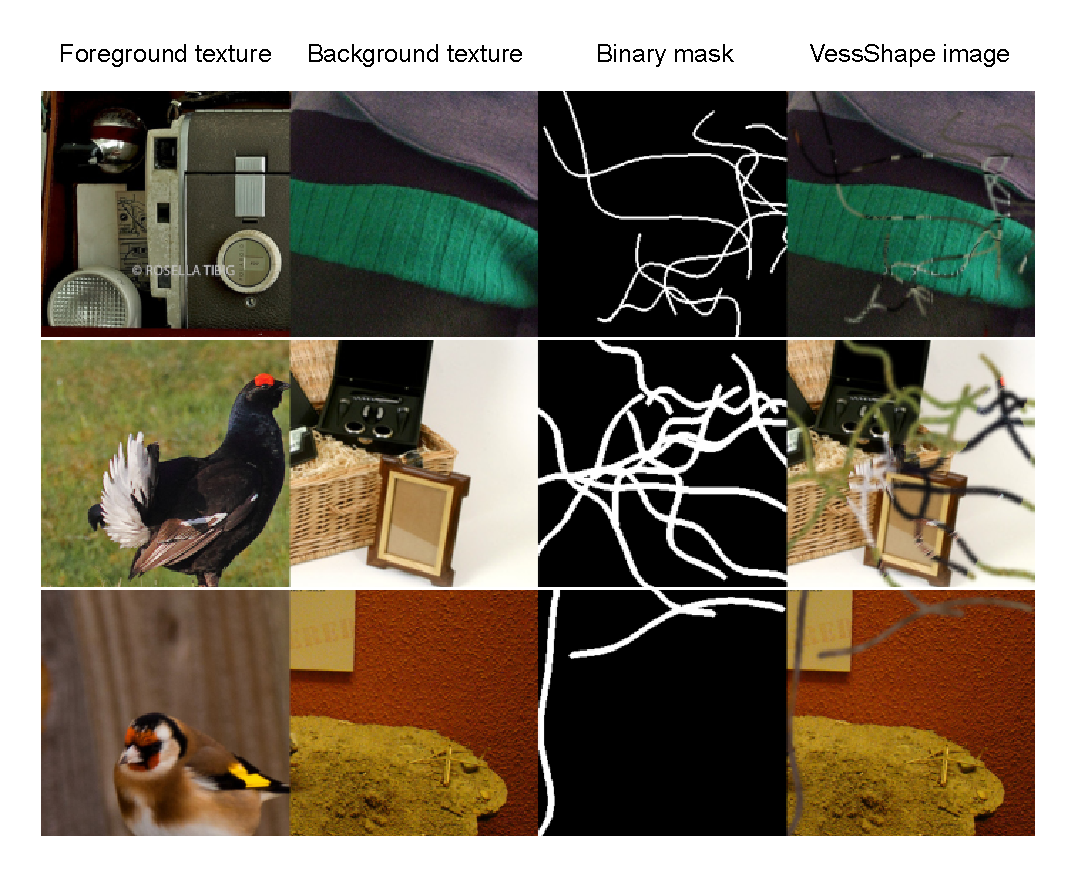
\includegraphics[width=\columnwidth]{figures/results/vessshape_sample.pdf}
    \caption{Examples of ImageNet samples, synthetic geometry and respective VessShape images. The ImageNet samples are used as textures for the synthetic binary masks, defining the respective VessShape image.}
    \label{f:vessshape_sample}
\end{figure}

\subsection{Real-world data for validation}

To quantify the usefulness of the shape bias introduced by the VessShape dataset, we consider two blood vessel datasets: DRIVE and VessMAP. The DRIVE dataset~\cite{} serves as a popular standard for benchmarking retinal vessel segmentation algorithms and is composed of 40 fundus photographs split into 20 for training and 20 for testing, each measuring 584×565 pixels. The VessMAP dataset consists of 100 images, 256×256 pixels each, acquired via fluorescence microscopy of the mouse cortex. It was curated to include a variety of challenging vascular features, such as inconsistent noise and contrast levels, different vessel sizes, prominent imaging artifacts, and intensity fluctuations within vessel structures.

The two datasets originate from fundamentally different imaging modalities, resulting in distinct characteristics. The fundus images in DRIVE, which capture the entire retina, possess a clear global structure that includes landmarks like the optic disk. The samples also contain many very thin vessels which are challenging to segment. In contrast, the VessMAP images are highly magnified views of small cortical areas and have no discernible global organization. The borders of the vessels are generally less defined than the vessels from DRIVE. Another key difference is that, without any processing, the vessels in VessMAP are bright with dark backgrounds while the vessels in DRIVE are dark with bright backgrounds. Figure \ref{f:drive_vessmap_samples} shows one sample from each dataset.

\begin{figure}[tbp]
    \centering
    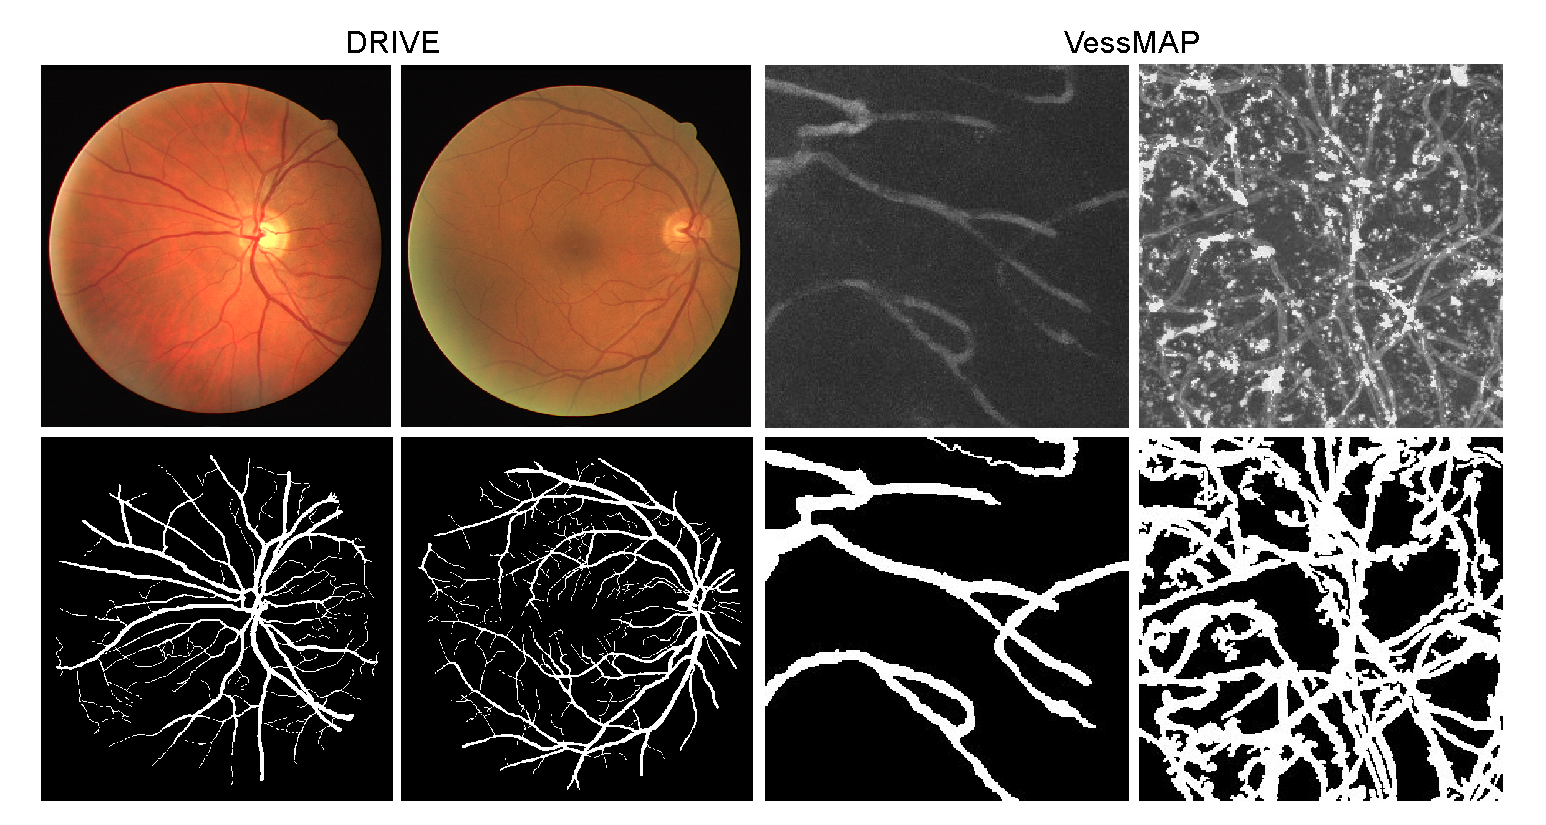
\includegraphics[width=\columnwidth]{figures/results/drive_vessmap_samples.pdf}
    \caption{Samples from the DRIVE and VessMAP datasets and their respective ground-truth masks.}
    \label{f:drive_vessmap_samples}
\end{figure}

\subsection{Model architectures and training strategies}

We adopt an encoder–decoder U-Net design, that is, the decoder is symmetrical to the encoder and the model contains skip connections between different encoder-decoder stages. Two models ar compared, one with a ResNet18 and the other with a ResNet50 encoder \cite{he2016deep}. The models were instantiated from the \textit{Segmentation Models Pytorch} Python package\footnote{\url{https://github.com/qubvel/segmentation_models.pytorch}}.

Two training scenarios are considered. In the first, training is done from scratch separately on the DRIVE and VessMAP datasets to establish a baseline. The second scenario consists of pre-training on the VessShape dataset and fine-tuning on DRIVE and VessMAP to measure the transferability and sample efficiency of the learned representations. These two scenarios involve three distinct training procedures: i) training from scratch on natural datasets; ii) pre-training on VessShape and iii) fine-tuning on real-world data. These procedures are described next.

\subsection{Training from scratch on natural datasets}

\subsection{Pre-training on VessShape}

The pre-training on VessShape aims to expose the model to a wide variety of tubular geometries while keeping texture as a secondary cue, which tends to benefit the segmentation of thin structures. The model is trained to minimize the average loss over a large number of samples drawn from the synthetic dataset

Concretely, we pre-train two U-Net models, one with a ResNet18 encoder and another with a ResNet50 encoder. We refer to them as VSUNet18 and VSUNet50, respectively. The training stream intentionally exposes the model to vessel-like geometries, while textures keep changing in the background. This narrative of abundant shapes and shifting appearances nudges the network to rely less on superficial texture cues and more on geometric regularities that matter for connectivity and thin-structure recovery. Below, we detail the VSUNet50 setup and summarize its performance on VessShape.

\begin{table}[t]
    \caption{Pre-training hyperparameters on VessShape.}
    \label{tab:vs_hparams}
    \centering
    \begingroup
    \small
    \setlength{\tabcolsep}{6pt}
    \renewcommand{\arraystretch}{1.15}
    \begin{tabular}{l r r}
        \hline
        	\textbf{Hyperparameter} & \textbf{VSUNet50} & \textbf{VSUNet18} \\
        \hline
        Batch size & 96 & 192 \\
        Learning rate & 1.0e-3 & 1.0e-2 \\
        Learning rate decay & 0.0 & 0.0 \\
        Weight decay & 1.0e-4 & 0.0 \\
        Imgs/epoch & 50{,}000 & 50{,}000 \\
        Max epochs & 3000 & 1000 \\
        \hline
    \end{tabular}
    \endgroup
\end{table}


\subsection{Fine-tuning on natural datasets}

- Datasets (VessMAP e DRIVE)

- Procedure

\begin{table}[t]
    \caption{Performance of VSUNet variants after pre-training on VessShape.}
    \label{tab:vessshape_results}
    \centering
    \begingroup
    \small
    \setlength{\tabcolsep}{6pt}
    \renewcommand{\arraystretch}{1.15}
    \begin{tabular}{l r r}
        \hline
        	\textbf{Metric} & \textbf{VSUNet50} & \textbf{VSUNet18} \\
        \hline
        Dice & $0.861 \,\pm\, 0.022$ & $0.859 \,\pm\, 0.077$ \\
        Acc & $0.960 \,\pm\, 0.008$ & $0.956 \,\pm\, 0.037$ \\
        IoU & $0.758 \,\pm\, 0.032$ & $0.761 \,\pm\, 0.096$ \\
        Prec & $0.780 \,\pm\, 0.037$ & $0.774 \,\pm\, 0.096$ \\
        Rec & $0.964 \,\pm\, 0.012$ & $0.974 \,\pm\, 0.018$ \\
        \hline
    \end{tabular}
    \endgroup
\end{table}

\section{Results}
\label{s:results}

\begin{figure*}[tbp]
    \centering
    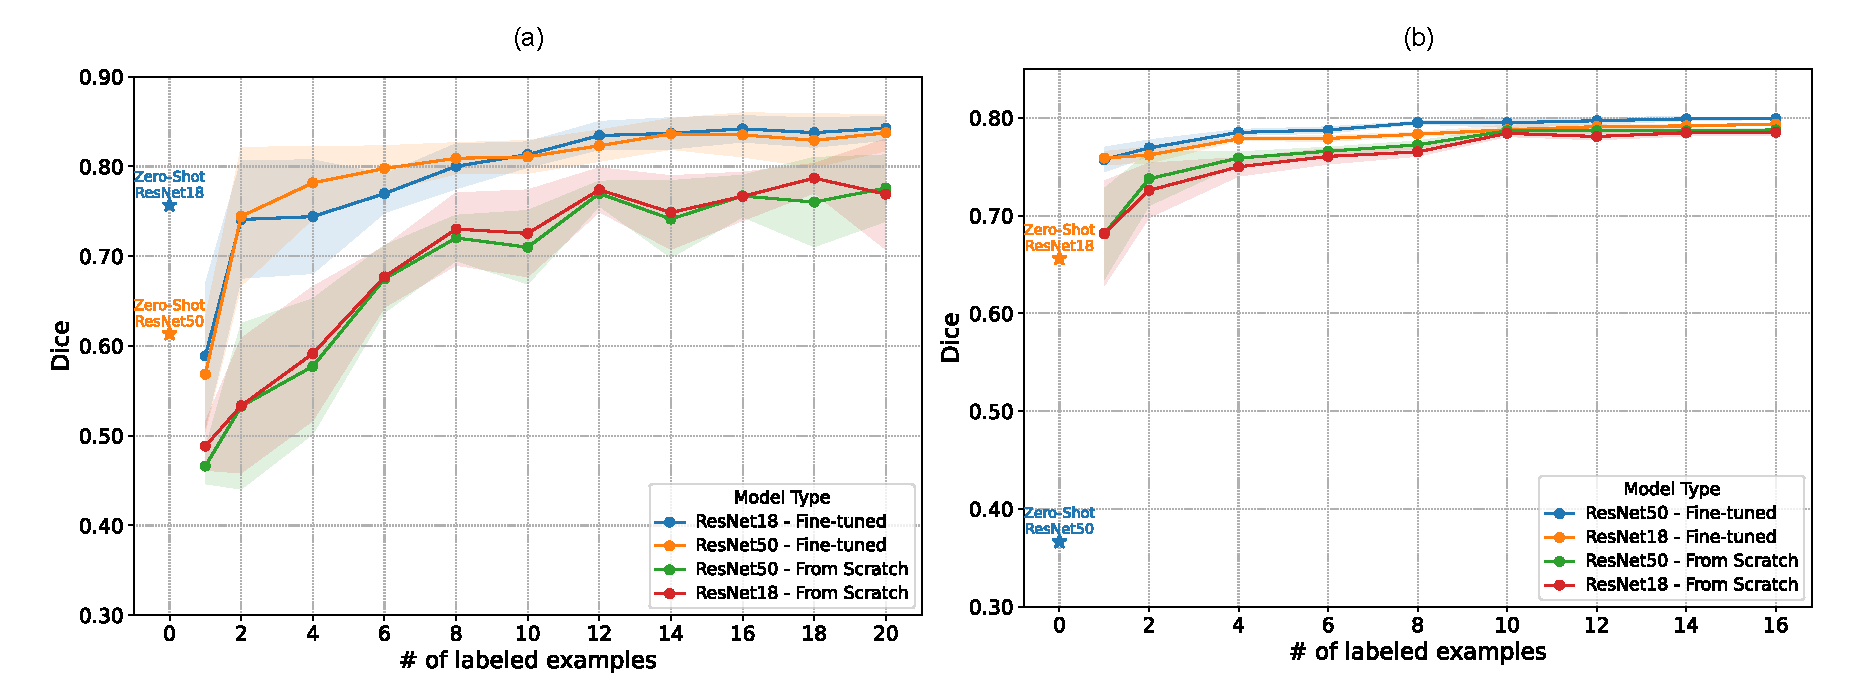
\includegraphics[width=\textwidth]{figures/results/results_charts.pdf}
    \caption{??.}
    \label{f:results_charts}
\end{figure*}


\begin{figure*}[tbp]
    \centering
    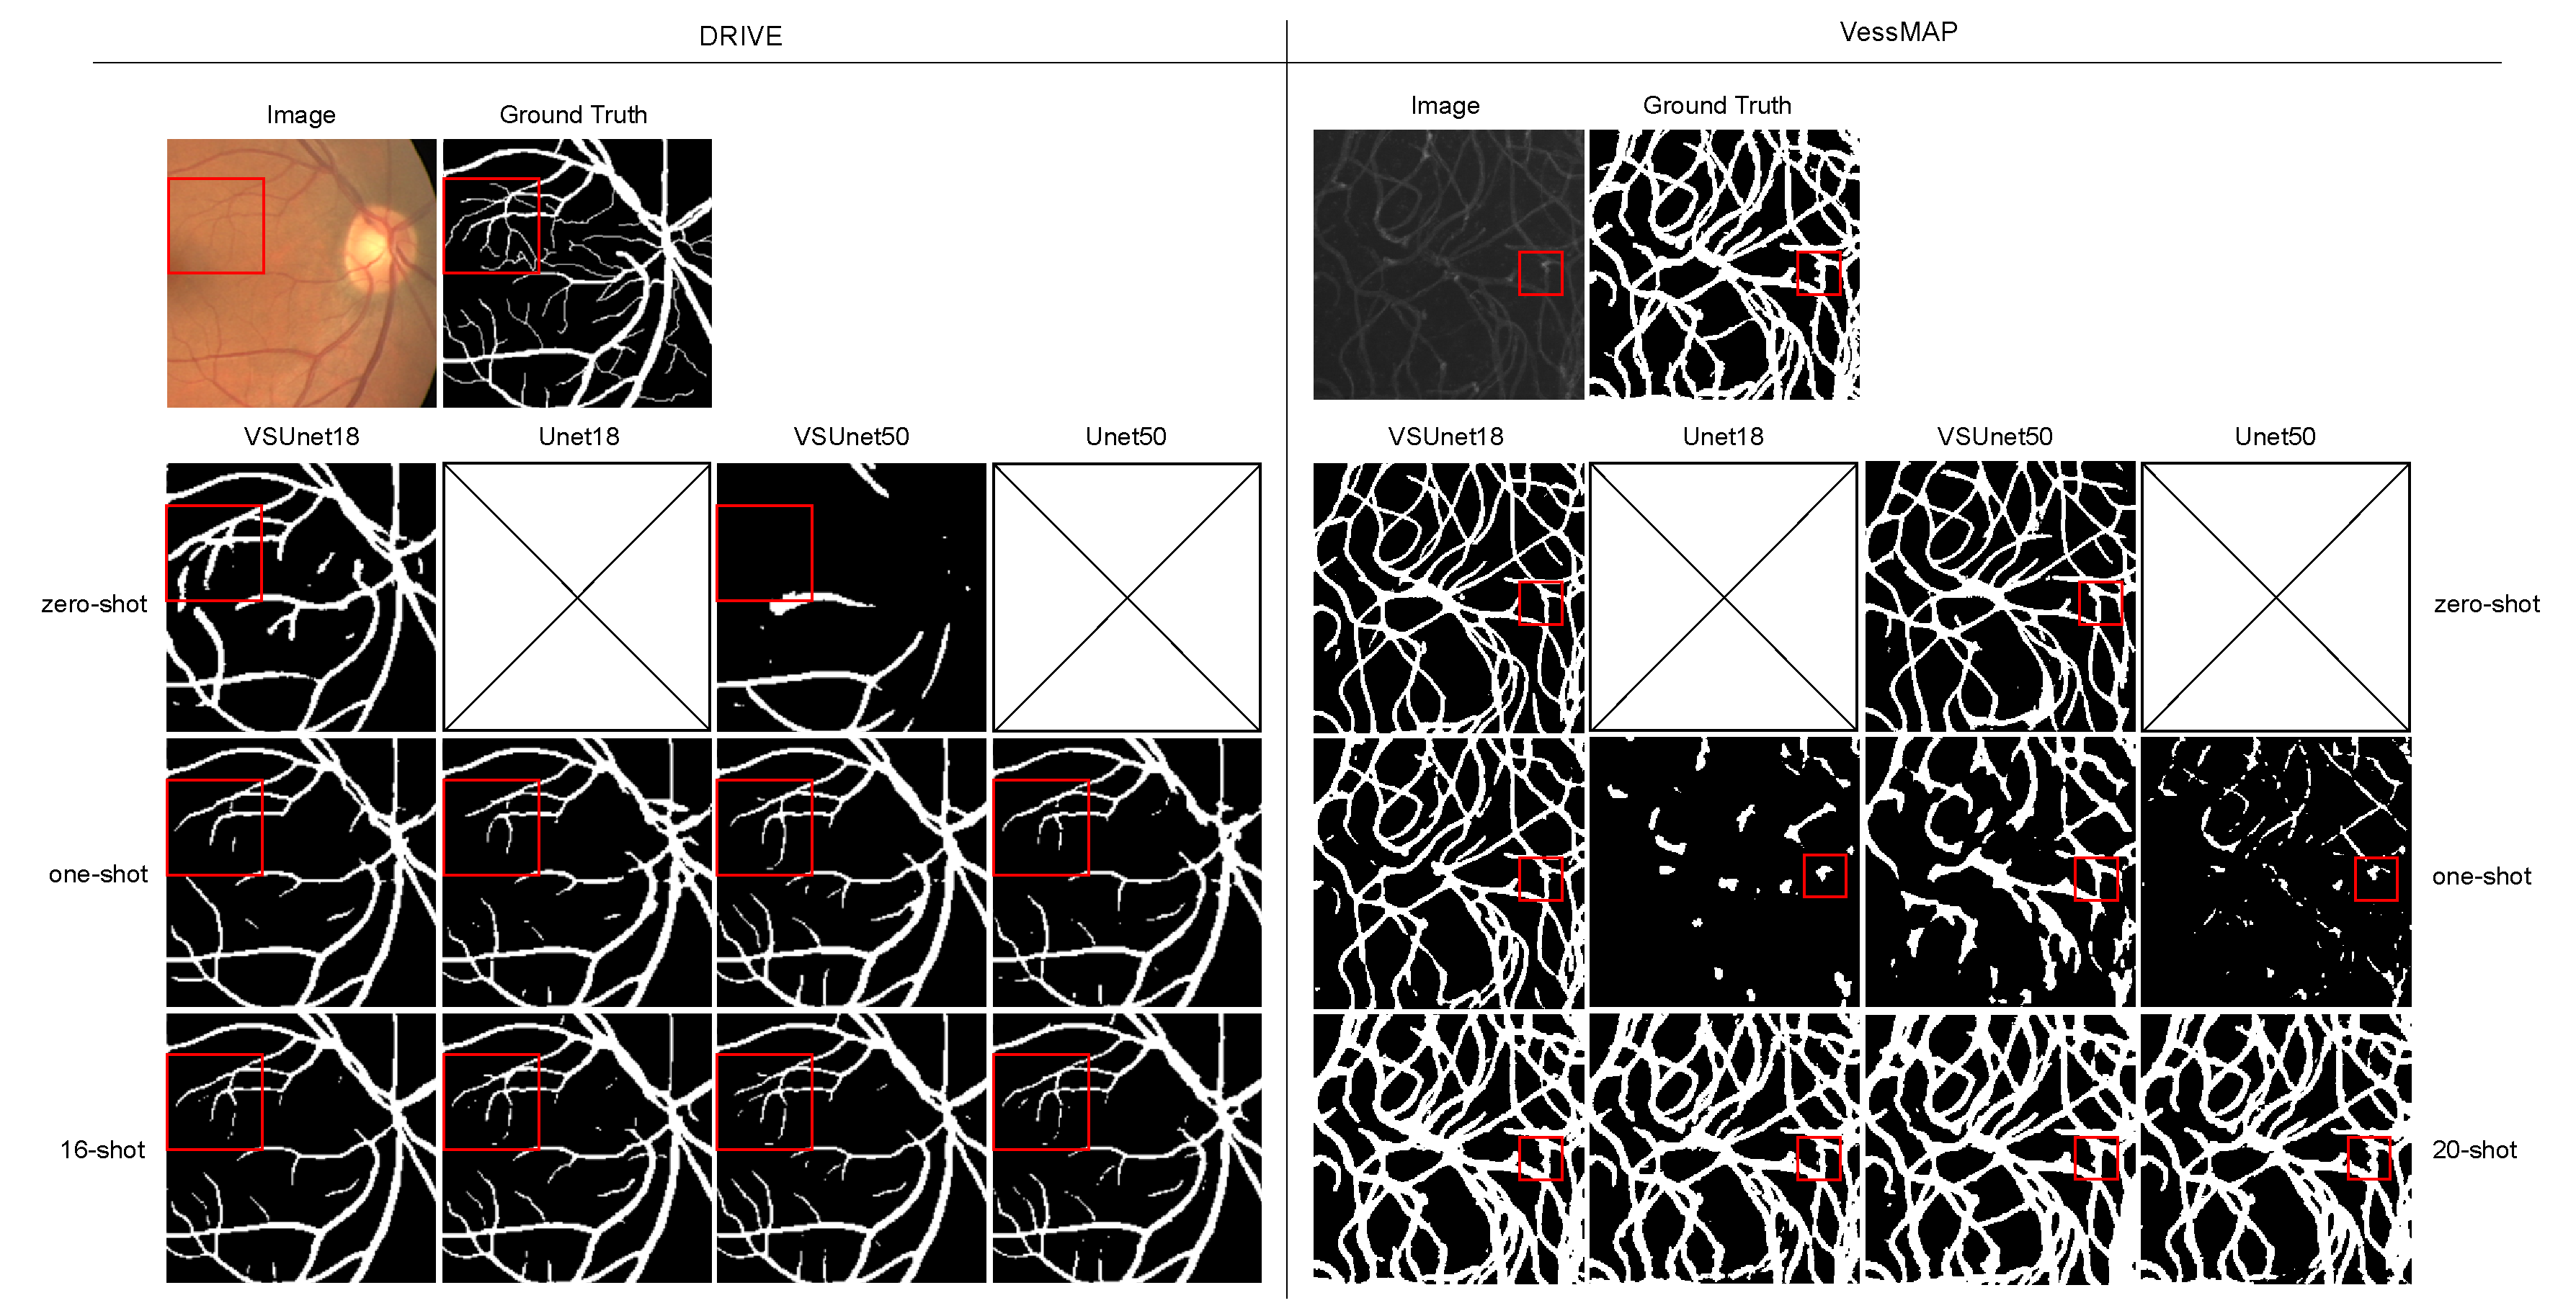
\includegraphics[width=\textwidth]{figures/results/results_fewshots.pdf}
    \caption{??.}
    \label{f:results_fewshots_drive}
\end{figure*}




% TODO:
% Argumentar que o nosso modelo é capaz de segmentar em zero-shot a forma do vaso, mesmo para VessMap que tem vasos com intensidade mais alta (branco), e DRIVE, com vasos com intensidade mais baixa(preto). 

% Combined VessMAP + DRIVE few-shot table
\begin{table*}[t]
    \caption{Few-shot and zero-shot segmentation on VessMAP and DRIVE. Values are mean $\pm$ standard deviation over repeated runs (fine-tuning for VSUNet models and training from scratch for U-Net baselines) evaluated on each dataset test set. Zero-shot rows come from a single pretrained inference (no deviation available).}
    \label{tab:combined_fewshot}
    \centering
    \begingroup
    \small
    \setlength{\tabcolsep}{4pt}
    \renewcommand{\arraystretch}{1.15}
    % Removed AUC column; merged Dataset cells with multirow
    \begin{tabular}{l r l r r r r r}
        \hline
        \textbf{Dataset} & \textbf{\#Examples} & \textbf{Model} & \textbf{Dice} & \textbf{Acc} & \textbf{IoU} & \textbf{Prec} & \textbf{Rec} \\
        \hline
        \multirow{10}{*}{DRIVE} & \multirow{2}{*}{0} & VSUNet18 & $0.656 \,\pm\, 0.000$ & $0.907 \,\pm\, 0.000$ & $0.490 \,\pm\, 0.000$ & $0.629 \,\pm\, 0.000$ & $0.699 \,\pm\, 0.000$ \\
         &  & VSUNet50 & $0.367 \,\pm\, 0.000$ & $0.888 \,\pm\, 0.000$ & $0.230 \,\pm\, 0.000$ & $0.728 \,\pm\, 0.000$ & $0.275 \,\pm\, 0.000$ \\
         \cline{2-8}
         & \multirow{4}{*}{1} & VSUNet18 & $0.759 \,\pm\, 0.007$ & $0.941 \,\pm\, 0.002$ & $0.612 \,\pm\, 0.009$ & $0.787 \,\pm\, 0.021$ & $0.741 \,\pm\, 0.019$ \\
         &  & VSUNet50 & $0.757 \,\pm\, 0.013$ & $0.939 \,\pm\, 0.006$ & $0.611 \,\pm\, 0.016$ & $0.773 \,\pm\, 0.046$ & $0.754 \,\pm\, 0.039$ \\
         &  & UNet18 & $0.682 \,\pm\, 0.054$ & $0.919 \,\pm\, 0.016$ & $0.523 \,\pm\, 0.058$ & $0.717 \,\pm\, 0.079$ & $0.690 \,\pm\, 0.118$ \\
         &  & UNet50 & $0.681 \,\pm\, 0.046$ & $0.916 \,\pm\, 0.031$ & $0.523 \,\pm\, 0.050$ & $0.722 \,\pm\, 0.099$ & $0.690 \,\pm\, 0.110$ \\
         \cline{2-8}
         & \multirow{4}{*}{16} & VSUNet18 & $0.794 \,\pm\, 0.000$ & $0.950 \,\pm\, 0.000$ & $0.658 \,\pm\, 0.000$ & $0.833 \,\pm\, 0.004$ & $0.762 \,\pm\, 0.003$ \\
         &  & VSUNet50 & $0.799 \,\pm\, 0.001$ & $0.952 \,\pm\, 0.000$ & $0.666 \,\pm\, 0.001$ & $0.846 \,\pm\, 0.003$ & $0.762 \,\pm\, 0.004$ \\
         &  & UNet18 & $0.785 \,\pm\, 0.003$ & $0.946 \,\pm\, 0.001$ & $0.647 \,\pm\, 0.004$ & $0.795 \,\pm\, 0.005$ & $0.781 \,\pm\, 0.004$ \\
         &  & UNet50 & $0.788 \,\pm\, 0.002$ & $0.947 \,\pm\, 0.001$ & $0.650 \,\pm\, 0.002$ & $0.807 \,\pm\, 0.006$ & $0.774 \,\pm\, 0.004$ \\
        \hline
        \multirow{10}{*}{VessMAP} & \multirow{2}{*}{0} & VSUNet18 & $0.757 \,\pm\, 0.000$ & $0.886 \,\pm\, 0.000$ & $0.616 \,\pm\, 0.000$ & $0.846 \,\pm\, 0.000$ & $0.696 \,\pm\, 0.000$ \\
         &  & VSUNet50 & $0.614 \,\pm\, 0.000$ & $0.817 \,\pm\, 0.000$ & $0.472 \,\pm\, 0.000$ & $0.746 \,\pm\, 0.000$ & $0.605 \,\pm\, 0.000$ \\
         \cline{2-8}
         & \multirow{4}{*}{1} & VSUNet18 & $0.589 \,\pm\, 0.080$ & $0.705 \,\pm\, 0.205$ & $0.455 \,\pm\, 0.088$ & $0.675 \,\pm\, 0.205$ & $0.738 \,\pm\, 0.148$ \\
         &  & VSUNet50 & $0.569 \,\pm\, 0.063$ & $0.708 \,\pm\, 0.203$ & $0.439 \,\pm\, 0.071$ & $0.683 \,\pm\, 0.208$ & $0.700 \,\pm\, 0.167$ \\
         &  & UNet18 & $0.488 \,\pm\, 0.027$ & $0.674 \,\pm\, 0.184$ & $0.362 \,\pm\, 0.032$ & $0.682 \,\pm\, 0.204$ & $0.622 \,\pm\, 0.210$ \\
         &  & UNet50 & $0.466 \,\pm\, 0.020$ & $0.665 \,\pm\, 0.181$ & $0.343 \,\pm\, 0.025$ & $0.674 \,\pm\, 0.206$ & $0.604 \,\pm\, 0.215$ \\
         \cline{2-8}
         & \multirow{4}{*}{20} & VSUNet18 & $0.843 \,\pm\, 0.013$ & $0.901 \,\pm\, 0.021$ & $0.739 \,\pm\, 0.018$ & $0.825 \,\pm\, 0.049$ & $0.888 \,\pm\, 0.048$ \\
         &  & VSUNet50 & $0.837 \,\pm\, 0.020$ & $0.905 \,\pm\, 0.025$ & $0.732 \,\pm\, 0.026$ & $0.851 \,\pm\, 0.032$ & $0.850 \,\pm\, 0.027$ \\
         &  & UNet18 & $0.769 \,\pm\, 0.062$ & $0.880 \,\pm\, 0.034$ & $0.645 \,\pm\, 0.075$ & $0.864 \,\pm\, 0.045$ & $0.737 \,\pm\, 0.094$ \\
         &  & UNet50 & $0.776 \,\pm\, 0.037$ & $0.880 \,\pm\, 0.035$ & $0.653 \,\pm\, 0.046$ & $0.855 \,\pm\, 0.041$ & $0.752 \,\pm\, 0.051$ \\
        \hline
    \end{tabular}
    \endgroup
\end{table*}



\section{Conclusion}
\label{s:conclusion}
% Trabalhos futuros: testar o modelo em imagens 3D

% One drawback of the method is that the network might not recognize vessels that do not follow the shape priors acquiried during training. For instance, stroke....


\section*{Funding}
C. H. Comin thanks FAPESP (grant no. 21/12354-8) for financial support. 


\bibliography{references}

\end{document}